\documentclass{article}

\usepackage{amsmath}
\usepackage{amsfonts}
\usepackage{amssymb}
\usepackage{textcomp, gensymb}
\usepackage[dvipsnames]{xcolor}
\usepackage[margin=0.5in]{geometry}
\usepackage[hidelinks]{hyperref}

\usepackage{tikz}
\usetikzlibrary{quantikz}
% \usepackage{blochsphere}

\usepackage{environ}
\NewEnviron{centerframebox}{\begin{center}\fbox{\parbox{0.92\textwidth}{\BODY}}\end{center}}

\let\oldphi\phi
\let\phi\varphi

\newcommand{\N}{\mathbb{N}}
\newcommand{\R}{\mathbb{R}}
\newcommand{\C}{\mathbb{C}}

\title{Quantum Algorithms \\ Exercise 2}
\author{
  AAAAAAAAAA AAAAAAA \\ \href{mailto:AAAAAAAAAAAAAAAAAAAA}{AAAAAAAAAAAAAAAAAAAA} \and
  Chuong Dinh Le \\ \href{mailto:s56dle@uni-bonn.de}{s56dle@uni-bonn.de} \and
  Paul Berners \\ \href{mailto:s6plbern@uni-bonn.de}{s6plbern@uni-bonn.de} \and
  Fynn Osterfeld \\ \href{mailto:s6fyoste@uni-bonn.de}{s6fyoste@uni-bonn.de}
}

\begin{document}
  \maketitle

  \setcounter{section}{2}
  \subsection{The Harmonic Oscillator}
  \begin{centerframebox}
    Consider the following Hamiltonian in $x$-representation for a quadratic potential:

    \[ \hat{H}(x) = -\frac{\hbar^{2}}{2m}\frac{d^{2}}{d x^{2}}+\frac{1}{2}m\omega^{2}x^{2} \]

    \begin{itemize}
      \item Show that the following wave function given by the normal distribution (Gaussian distribution) solves the time-independent Schrödinger equation:
      \[ \psi(x) = \psi_0\exp\left[-\frac{m\omega}{2\hbar}x^{2}\right] \]
      \item Calculate the corresponding energy $E$ as a function of $\omega$.
      \item Calculate $\psi_0$ such that $\psi$ is normalized: $\langle\psi|\psi\rangle = \int\psi^{*}(x)\,\psi(x)\, dx = 1$ \\
      Hint: ${\int}_{-\infty}^{\infty}\exp[-x^{2}] dx = {\sqrt{\pi}}$.
      \item Calculate the expectation values of the position $x$ and the momentum operator $\hat{p} = -i\hbar \frac{d}{d x}$
      \[ \bar{x} = \langle\psi|\hat{x}|\psi\rangle = \int\psi^{*}(x) x\, \psi(x)\, dx \]
      \[ \bar{p} = \langle\psi|\hat{p}|\psi\rangle = \int\psi^{*}(x) \hat{p}\, \psi(x)\, dx \]
    \end{itemize}

    Hint: use symmetry.
  \end{centerframebox}
  Show that $\psi$ satisfies the Schrödinger equation:
  \begin{align*}
      \hat{H}\psi(x) &= \left(-\frac{\hbar^2}{2m}\frac{\partial^2}{\partial x^2} + \frac{1}{2}m\omega^2x^2\right)\left(\psi_0\exp\left(-\frac{m\omega}{2\hbar}x^2\right)\right)\\
      &= \frac{1}{2}\psi_0\left(-\frac{\hbar^2}{m}\frac{\partial^2}{\partial x^2}\exp\left(-\frac{m\omega}{2\hbar}x^2\right) + m\omega^2x^2\exp\left(-\frac{m\omega}{2\hbar}x^2\right)\right)\\
      &= \frac{1}{2}\psi_0\left(-\frac{\hbar^2}{m}\frac{\partial}{\partial x}\left(-\frac{m\omega}{2\hbar}\cdot 2x\cdot\exp\left(-\frac{m\omega}{2\hbar}x^2\right)\right)  + m\omega^2x^2\exp\left(-\frac{m\omega}{2\hbar}x^2\right)\right)\\
      &= \frac{1}{2}\psi_0\left(\frac{\hbar^2}{m}\frac{m\omega}{2\hbar}\cdot 2\cdot \frac{\partial}{\partial x}\left(x\cdot\exp\left(-\frac{m\omega}{2\hbar}x^2\right)\right)  + m\omega^2x^2\exp\left(-\frac{m\omega}{2\hbar}x^2\right)\right)\\
      &= \frac{1}{2}\psi_0\omega\left(\hbar\frac{\partial}{\partial x}\left(x\cdot\exp\left(-\frac{m\omega}{2\hbar}x^2\right)\right)  + m\omega x^2\exp\left(-\frac{m\omega}{2\hbar}x^2\right)\right)\\
      &= \frac{1}{2}\psi_0\omega\left(\hbar\left(\exp\left(-\frac{m\omega}{2\hbar}x^2\right) + x\cdot\left(-\frac{m\omega}{2\hbar}\cdot 2x\right)\exp\left(-\frac{m\omega}{2\hbar}x^2\right)\right)  + m\omega x^2\exp\left(-\frac{m\omega}{2\hbar}x^2\right)\right)\\
      &= \frac{1}{2}\psi_0\omega\left(\hbar\left(1 + x\cdot\left(-\frac{m\omega}{2\hbar}\cdot 2x\right)\right)  + m\omega x^2\right)\exp\left(-\frac{m\omega}{2\hbar}x^2\right)\\
      &= \frac{1}{2}\omega\left(\hbar - \hbar\frac{m\omega}{\hbar}\cdot x^2  + m\omega x^2\right)\psi(x)\\
      &= \frac{1}{2}\omega\hbar\psi(x)
  \end{align*}
  So with $E := \frac{1}{2}\omega\hbar$ we have $\hat{H}\psi(x) = E\psi(x)$.\\
  $E$ as a function of $\omega$ consequently is:
  \begin{align*}
      E(\omega) &= \frac{1}{2}\hbar\omega
  \end{align*}
  For $\langle\psi|\psi\rangle = \int\psi^{*}(x)\,\psi(x)\, dx = 1$ to hold we need the additional condition $\omega \neq 0$.\\
  First calculate $\langle\psi|\psi\rangle$:
  \begin{align*}
      \langle\psi|\psi\rangle &= \int_{-\infty}^\infty\overline{\psi(x)}\psi(x)dx\\
      &= \int_{-\infty}^\infty\overline{\left(\psi_0\exp\left(-\frac{m\omega}{2\hbar}x^2\right)\right)}\left(\psi_0\exp\left(-\frac{m\omega}{2\hbar}x^2\right)\right)dx\\
      &= |\psi_0|^2\int_{-\infty}^\infty\left(\exp\left(-\frac{m\omega}{2\hbar}x^2\right)\right)\left(\exp\left(-\frac{m\omega}{2\hbar}x^2\right)\right)dx\\
      &= |\psi_0|^2\int_{-\infty}^\infty\exp\left(-\frac{m\omega}{\hbar}x^2\right)dx&|\,\,\text{substitute:}\quad t = \sqrt{\frac{m\omega}{\hbar}}x\\
      &= |\psi_0|^2\frac{1}{\sqrt{\frac{m\omega}{\hbar}}}\int_{-\infty}^\infty\exp\left(-t^2\right)dt\\
      &= |\psi_0|^2\sqrt{\frac{\hbar}{m\omega}}\sqrt{\pi}\\
      &= |\psi_0|^2\sqrt{\frac{\hbar\pi}{m\omega}}
  \end{align*}
  Now solve $\langle\psi|\psi\rangle = 1$ for $\psi_0$:
  \begin{align*}
      1 &= \langle\psi|\psi\rangle\\
      1 &= |\psi_0|^2\sqrt{\frac{\hbar\pi}{m\omega}}\\
      |\psi_0|^2 &= \sqrt{\frac{m\omega}{\hbar\pi}}\\
      |\psi_0| &= \sqrt{\sqrt{\frac{m\omega}{\hbar\pi}}}
  \end{align*}
  So for $\psi_0 = \sqrt[4]{\frac{m\omega}{\hbar\pi}}$ the function $\psi$ is normalized.\\\\
  Using the hint, one can notice that $x\exp\left(-x^2\right)$ is a point-symmetric function relative to $(0, 0)$, which makes the indefinite integral $\int_{-\infty}^\infty x\exp\left(-x^2\right)dx$ trivial, i.e. $= 0$.\\
  Knowing this, we can easily calculate both $\Bar{x}$ and $\Bar{p}$:
  \begin{align*}
      \Bar{x} &= \langle\psi|\hat{x}|\psi\rangle\\
      &= \int_{-\infty}^\infty\overline{\psi(x)}x\psi(x)dx\\
      &= \int_{-\infty}^\infty\overline{\left(\psi_0\exp\left(-\frac{m\omega}{2\hbar}x^2\right)\right)}x\left(\psi_0\exp\left(-\frac{m\omega}{2\hbar}x^2\right)\right)dx\\
      &= |\psi_0|^2\int_{-\infty}^\infty x\exp\left(-\frac{m\omega}{\hbar}x^2\right)dx\\
      &= |\psi_0|^2\frac{1}{\sqrt{\frac{m\omega}{\hbar}}}\int_{-\infty}^\infty \sqrt{\frac{m\omega}{\hbar}}x\exp\left(-\frac{m\omega}{\hbar}x^2\right)dx\\
      &= |\psi_0|^2\sqrt{\frac{\hbar}{m\omega}}\int_{-\infty}^\infty t\exp\left(-t^2\right)dt\\
      &= |\psi_0|^2\sqrt{\frac{\hbar}{m\omega}}\cdot 0\\
      &= 0
  \end{align*}
  \begin{align*}
      \Bar{p} &= \langle\psi|\hat{p}|\psi\rangle\\
      &= \int_{-\infty}^\infty\overline{\psi(x)}\hat{p}\psi(x)dx\\
      &= \int_{-\infty}^\infty\overline{\left(\psi_0\exp\left(-\frac{m\omega}{2\hbar}x^2\right)\right)}\left(-i\hbar\frac{d}{dx}\right)\left(\psi_0\exp\left(-\frac{m\omega}{2\hbar}x^2\right)\right)dx\\
      &= |\psi_0|^2(-i\hbar)\int_{-\infty}^\infty \exp\left(-\frac{m\omega}{2\hbar}x^2\right) \frac{d}{dx} \exp\left(-\frac{m\omega}{2\hbar}x^2\right) dx\\
      &= |\psi_0|^2(-i\hbar)\int_{-\infty}^\infty \exp\left(-\frac{m\omega}{2\hbar}x^2\right) \left(-\frac{m\omega}{\hbar}x\right) \exp\left(-\frac{m\omega}{2\hbar}x^2\right) dx\\
      &= |\psi_0|^2 im\omega \int_{-\infty}^\infty x\exp\left(-\frac{m\omega}{\hbar}x^2\right)dx\\
      &= |\psi_0|^2 im\omega \cdot 0\\
      &= 0
  \end{align*}

  \subsection{The Two State System}
  \begin{centerframebox}
    Consider the two-state system from the lecture 2 with $\hat{H} = \mu B \sigma_x$ and the initial state $|\psi(0)\rangle = |0\rangle$.
    In the lecture, it was derived that the wave function is of the form
    \[ \psi(t) = \begin{pmatrix}
      \cos(\omega t) \\
      -i\sin(\omega t)
    \end{pmatrix}, \]
    where $\omega={\frac{\mu B}{\hbar}}$.

    \begin{itemize}
      \item Show that the expectation of
      \[ \sigma_x = \begin{pmatrix}
        0 & 1 \\
        1 & 0
      \end{pmatrix} \]
      is given by
      \[\overline{\sigma_{x}} = \langle\psi(t)|\,\sigma_{x}\,|\psi(t)\rangle = 0.\]
    \end{itemize}
  \end{centerframebox}
  You can use $\sin(\alpha - \beta) = \sin(\alpha)\cos(\beta) - \cos(\alpha)\sin(\beta)$ to calculate $\overline{\sigma_x}$:
  \begin{align*}
      \overline{\sigma_{x}} &= \langle\psi(t)|\,\sigma_{x}\,|\psi(t)\rangle\\
      &= \overline{\begin{pmatrix}\cos(\omega t)\\-i\sin(\omega t)\end{pmatrix}}^T\begin{pmatrix}0&1\\1&0\end{pmatrix}\begin{pmatrix}\cos(\omega t)\\-i\sin(\omega t)\end{pmatrix}\\
      &= \begin{pmatrix}\cos(\omega t)&i\sin(\omega t)\end{pmatrix}\begin{pmatrix}-i\sin(\omega t)\\\cos(\omega t)\end{pmatrix}\\
      &= -i\cos(\omega t)\sin(\omega t) + i\sin(\omega t)\cos(\omega t)\\
      &= i(\sin(\omega t)\cos(\omega t) - \cos(\omega t)\sin(\omega t))\\
      &= i\sin(\omega t - \omega t)\\
      &= i\sin(0)\\
      &= 0
  \end{align*}

  \subsection{The Y-Basis}
  \begin{centerframebox}
    In the lecture, the Z- and X-basis for the vector space of qubit states were presented.

    \begin{itemize}
      \item Prove that the following qubit states are the Y-basis.
      \[ |R\rangle = \frac{1}{\sqrt{2}} (|0\rangle+i\,|1\rangle) \]
      \[ |L\rangle = \frac{1}{\sqrt{2}} (|0\rangle-i\,|1\rangle) \]
      \item Provide a quantum algorithm composed of gates in order to put a qubit initialized with $|0\rangle$
      into $|R\rangle$ and a qubit initialized with $|1\rangle$ into $|L\rangle$. Draw the corresponding quantum circuit.
      \item Draw the states $|R\rangle$ and $|L\rangle$ on a Bloch sphere.
    \end{itemize}
  \end{centerframebox}
  First, consider $Y = \begin{pmatrix}0&-i\\i&0\end{pmatrix}$. We have to prove that $|R\rangle$ and $|L\rangle$ are the eigenvalues of $Y$:
  \begin{align*}
      Y|R\rangle &= Y\frac{1}{\sqrt{2}}\left(\begin{pmatrix}1\\0\end{pmatrix}+i\begin{pmatrix}0\\1\end{pmatrix}\right)\\
      &= \frac{1}{\sqrt{2}}\left(Y\begin{pmatrix}1\\0\end{pmatrix} + iY\begin{pmatrix}0\\1\end{pmatrix}\right)\\
      &= \frac{1}{\sqrt{2}}\left(\begin{pmatrix}0\\i\end{pmatrix} + i\begin{pmatrix}-i\\0\end{pmatrix}\right)\\
      &= \frac{1}{\sqrt{2}}\left(i\begin{pmatrix}1\\0\end{pmatrix} + \begin{pmatrix}1\\0\end{pmatrix}\right)\\
      &= |R\rangle
  \end{align*}
  \begin{align*}
      Y|L\rangle &= Y\frac{1}{\sqrt{2}}\left(\begin{pmatrix}1\\0\end{pmatrix}-i\begin{pmatrix}0\\1\end{pmatrix}\right)\\
      &= \frac{1}{\sqrt{2}}\left(Y\begin{pmatrix}1\\0\end{pmatrix} - iY\begin{pmatrix}0\\1\end{pmatrix}\right)\\
      &= \frac{1}{\sqrt{2}}\left(\begin{pmatrix}0\\i\end{pmatrix} - i\begin{pmatrix}-i\\0\end{pmatrix}\right)\\
      &= \frac{1}{\sqrt{2}}\left(i\begin{pmatrix}0\\1\end{pmatrix} - \begin{pmatrix}1\\0\end{pmatrix}\right)\\
      &= -|L\rangle
  \end{align*}
  This makes $\{ |R\rangle, |L\rangle\}$ a $Y$-basis.\\\\

  The following matrix fits the desired properties:
  \begin{align*}
      U_{RL} :&= \frac{1}{\sqrt{2}}\begin{pmatrix}1&1\\i&-i\end{pmatrix}\\
      U_{RL} &= SH\\
      &= \begin{pmatrix}1&0\\0&i\end{pmatrix}\frac{1}{\sqrt{2}}\begin{pmatrix}1&1\\1&-1\end{pmatrix}\\
      &= \frac{1}{\sqrt{2}}\begin{pmatrix}1&1\\i&-i\end{pmatrix}
  \end{align*}
  Proof of $U_{RL}|0\rangle = |R\rangle$ and $U_{RL}|1\rangle = |L\rangle$ is given by seeing that $U_{RL}$ is just a concatenation of the two:
  \begin{align*}
      U_{RL} &= \left(|R\rangle|L\rangle\right)\\
      &= \begin{pmatrix}\frac{1}{\sqrt{2}}\begin{pmatrix}1\\i\end{pmatrix}&\frac{1}{\sqrt{2}}\begin{pmatrix}1\\-i\end{pmatrix}\end{pmatrix}\\
      &= \frac{1}{\sqrt{2}}\begin{pmatrix}1&1\\i&-i\end{pmatrix}
  \end{align*}
  The corresponding quantum circuit would be:\\
  \begin{center}
      \begin{quantikz}
          \lstick{\ket{\psi}}&\gate{H}&\gate{S}&\meter{}
      \end{quantikz}
  \end{center}
  or just:
  \begin{center}
      \begin{quantikz}
          &\gate{H}&\gate{S}&
      \end{quantikz}
  \end{center}
  $|R\rangle$ and $|L\rangle$ on the Bloch sphere:
  \begin{center}
    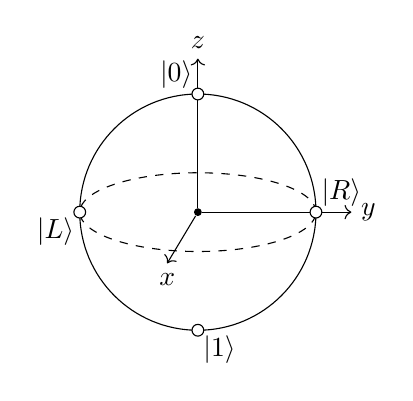
\begin{tikzpicture}[
      circ/.style={shape=circle, fill=white, node contents=, draw, outer sep=0pt, inner sep=1.5pt},
      label distance=-1.5mm
    ]
      \def\r{3/2}
      \def\axisext{1.3}

      % Bloch vector
      \draw (0,0) node[circle, fill, inner sep=1] (orig) {};

      % Sphere
      \draw (orig) circle (\r);
      \draw[dashed] (orig) ellipse ({\r} and \r/3);

      % Axes
      \draw[->] (orig) -- ++(-\r/5*\axisext, -\r/3*\axisext) node[below] (x1) {$x$};
      \draw[->] (orig) -- ++(\r*\axisext, 0) node[right] (x2) {$y$};
      \draw[->] (orig) -- ++(0, \r*\axisext) node[above] (x3) {$z$};

      \draw (0, \r) node[circ, label=above left:$|0\rangle$];
      \draw (0, -\r) node[circ, label=below right:$|1\rangle$];
      \draw (-\r, 0) node[circ, label=below left:$|L\rangle$];
      \draw (\r, 0) node[circ, label=above right:$|R\rangle$];
    \end{tikzpicture}
  \end{center}
\end{document}
